\documentclass [dvipdfmx,11pt]{beamer}
\usepackage{bxdpx-beamer}
\usepackage{pxjahyper}
\usepackage{amsmath}
\usepackage{bm}
\usepackage{minijs}
\usepackage{tikz}
\usepackage{multicol}
\usepackage{amssymb}
%\usepackage{otf}
%\renewcommand{\kanjifamilydefault}{\gtdefault}
%%% Beamer
%\AtBeginDvi{\special{pdf:tounicode EUC-UCS2}}
%\usetheme{Madrid}
%\usetheme{Copenhagen}
\usetheme{Warsaw}
% \renewcommand{\kanjifamilydefault}{\gtdefault}
\usefonttheme{structurebold}
%\usefonttheme{professionalfonts}
\setbeamertemplate{blocks}[shadow=true,rounded]
% \setbeamercolor{structure}{fg=blue!60!black}
\setbeamercolor{structure}{fg=blue!50!black}
\setbeamercolor{item projected}{fg=black,bg=blue!20!white}
%\setbeamercolor{alerted text}{fg=red!80!black}
\setbeamercolor{alerted text}{fg=red!70!black}
\setbeamertemplate{navigation symbols}{}
\useoutertheme[subsection=false]{miniframes}
\setbeamertemplate{footline}[frame number]
%%% Tikz
\usetikzlibrary{intersections, calc, arrows}
\setbeamertemplate{navigation symbols}{}
\setbeamertemplate{itemize item}[circle]
\setbeamersize{text margin left=1.5em,text margin right=1.5em}
\setlength{\abovedisplayskip}{0pt} % 上部のマージン
\setlength{\belowdisplayskip}{0pt} % 下部のマージン
\setlength{\columnsep}{0pt}
%
%
%
% footer setting %
\makeatother
\setbeamertemplate{footline}
{
    \leavevmode%
    \hbox{%
        \begin{beamercolorbox}[wd=.4\paperwidth,ht=2.25ex,dp=1ex,center]{author in head/foot}%
            \usebeamerfont{author in head/foot}\insertshortauthor
        \end{beamercolorbox}%
        \begin{beamercolorbox}[wd=.6\paperwidth,ht=2.25ex,dp=1ex,center]{title in head/foot}%
            \usebeamerfont{title in head/foot}\hspace*{1ex} \insertshorttitle\hspace*{2em}
            \textbf{ \insertframenumber{} / \inserttotalframenumber } \hspace*{1ex}
    \end{beamercolorbox}}%
    \vskip0pt%
}
\makeatletter
% exclude apprendix slides from framenumber %
\newcommand{\backupbegin}{
    \newcounter{framenumberappendix}
    \setcounter{framenumberappendix}{\value{framenumber}}
}
\newcommand{\backupend}{
    \addtocounter{framenumberappendix}{-\value{framenumber}}
    \addtocounter{framenumber}{\value{framenumberappendix}}
}


%%%%%%%%%%%%%%%%%%%%%%%%%%%%%%%%%%%%%%%%%%%%%%%%%%%%%%%%%%%%%%%%
% User-defined Macro
%%%%%%%%%%%%%%%%%%%%%%%%%%%%%%%%%%%%%%%%%%%%%%%%%%%%%%%%%%%%%%%%
\newcommand{\compress}{\itemsep0pt\parsep0pt\parskip0pt\partopsep0pt}
% \newcommand{\compress}{\itemsep1pt plus1pt\parsep0pt\parskip0pt}
% \newcommand{\code}[1]{\lstinline[basicstyle=\ttfamily]{#1}}
\newcommand{\gringo}{\textit{gringo}}
\newcommand{\clasp}{\textit{clasp}}
\newcommand{\clingo}{\textit{clingo}}
\newcommand{\teaspoon}{\textit{teaspoon}}
\newcommand{\sat}{\textsf{SAT}}
\newcommand{\unsat}{\textsf{UNSAT}}
% \newcommand{\web}[2]{\href{#1}{#2\ \raisebox{-0.15ex}{\beamergotobutton{Web}}}}
% \newcommand{\doi}[2]{\href{#1}{#2\ \raisebox{-0.15ex}{\beamergotobutton{DOI}}}}
% \newcommand{\weblink}[1]{\web{#1}{#1}}
% \newcommand{\imp}{\mathrel{\Rightarrow}}
% \newcommand{\Iff}{\mathrel{\Leftrightarrow}}
% \newcommand{\mybox}[1]{\fbox{\rule[.2cm]{0cm}{0cm}\mbox{${#1}$}}}
% \newcommand{\mycbox}[2]{\tikz[baseline]\node[fill=#1!10,anchor=base,rounded corners=2pt] () {#2};}
% \newcommand{\naf}[1]{\ensuremath{{\sim\!\!{#1}}}}
% \newcommand{\head}[1]{\ensuremath{\mathit{head}(#1)}}
% \newcommand{\body}[1]{\ensuremath{\mathit{body}(#1)}}
% \newcommand{\atom}[1]{\ensuremath{\mathit{atom}(#1)}}
% \newcommand{\poslits}[1]{\ensuremath{{#1}^+}}
% \newcommand{\neglits}[1]{\ensuremath{{#1}^-}}
% \newcommand{\pbody}[1]{\poslits{\body{#1}}}
% \newcommand{\nbody}[1]{\neglits{\body{#1}}}
% \newcommand{\Cn}[1]{\ensuremath{\mathit{Cn}(#1)}}
% \newcommand{\reduct}[2]{\ensuremath{#1^{#2}}}
% \newcommand{\OK}{\mbox{\textcolor{green}{\Pisymbol{pzd}{52}}}}
% \newcommand{\KO}{\mbox{\textcolor{red}{\Pisymbol{pzd}{56}}}}
% \newcommand{\code}[1]{\lstinline[basicstyle=\ttfamily]{#1}}
% \newcommand{\lw}[1]{\smash{\lower2.ex\hbox{#1}}}
\newcommand{\llw}[1]{\smash{\lower3.ex\hbox{#1}}}

\newenvironment{tableC}{%
  \scriptsize
  \renewcommand{\arraystretch}{0.9}
  \tabcolsep = 0.6mm
  % \begin{tabular}[t]{p{6mm}|rlr|rlr|rlr|rlr|rlr}\hline
  %   \multicolumn{1}{l|}{\llw{問題   }} &
  \begin{tabular}[t]{l|rlr|rlr|rlr|rlr|rlr}\hline
    \multicolumn{1}{l|}{\llw{問題}} &
    \multicolumn{3}{c|}{UD1} &
    \multicolumn{3}{c|}{UD2} &
    \multicolumn{3}{c|}{UD3} &
    \multicolumn{3}{c|}{UD4} &
    \multicolumn{3}{c}{UD5} \\
    & 
    \multicolumn{1}{c}{既知の} & & \multicolumn{1}{c|}{ASP} & 
    \multicolumn{1}{c}{既知の} & & \multicolumn{1}{c|}{ASP} & 
    \multicolumn{1}{c}{既知の} & & \multicolumn{1}{c|}{ASP} & 
    \multicolumn{1}{c}{既知の} & & \multicolumn{1}{c|}{ASP} & 
    \multicolumn{1}{c}{既知の} & & \multicolumn{1}{c}{ASP} \\
    & 
    ベスト & &  & 
    ベスト & &  & 
    ベスト & &  & 
    ベスト & &  & 
    ベスト & &  \\
    \hline
  }{%
    \hline
  \end{tabular}
}

%%%%%%%%%%%% my macro %%%%%%%%%%%%%%%%%
\newcommand{\alldifferent}{$alldifferent$}
%%%%%%%%%%%%%%%%%%%%%%%%%%%%%%%%%%%%%%%


\title{チャネリング制約を用いた\\ alldifferent 制約の SAT 符号化}
% \author{小菅脩司}
% \institute{名古屋大学}
\author{小菅 脩司\inst{1} \and 宋 剛秀\inst{2} \and 田村 直之\inst{2} \and 番原 睦則\inst{1}}
\institute{ \inst{1}名古屋大学 \ \  \inst{2}神戸大学 }
\date{情報処理学会第84回全国大会}
\begin{document}
\begin{frame} {}
    \titlepage
\end{frame}
%%%%%%%%%%%%%%%%%%%%%%%%%%%%%%%%%%%%%%




%%%%%%%%%%%%%%%%%%%%%%%%%%%%%%%%%%%%%%
% alldifferent制約
%%%%%%%%%%%%%%%%%%%%%%%%%%%%%%%%%%%%%%
\begin{frame}
    \frametitle{{\alldifferent}制約}
    \begin{alertblock}{}\centering
        \alert{\bm{$alldifferent(x_{1},x_{2},\ldots, x_{n})$}}\\[1em]
        \begin{itemize}
            \item 整数上の変数$x_{i}$が互いに異なることを表す制約である.
            \item 制約プログラミングにおける代表的なグローバル制約の一つである.
        \end{itemize}
    \end{alertblock}
    \begin{itemize}
        \item この制約は,
            $$\bigwedge_{1 \leq i < j \leq n} x_i \neq x_j$$
            を意味する.
        \item {\alldifferent}制約は,時間割問題,グラフ彩色問題,組合せデザイン
            など様々な制約充足問題に現れる.
        \item そのような問題に対し,{\alldifferent}制約を効率良く解くことは重要
            な研究課題である.
    \end{itemize}
\end{frame}



%%%%%%%%%%%%%%%%%%%%%%%%%%%%%%%%%%%%%%
% alldifferent制約の適用例
%%%%%%%%%%%%%%%%%%%%%%%%%%%%%%%%%%%%%%
\begin{frame}
    \frametitle{{\alldifferent}制約の適用例}
    \begin{block}{クイーングラフ彩色問題}
        $N$個ずつの$N$個のグループからなるクイーン (計$N^2$個) を,
        $N\times N$のチェス盤に,同じグループのクイーン同士が互いに取られ
        ないように配置する問題
    \end{block}
    \begin{exampleblock}{}\centering
        \begin{columns}
            \begin{column}{0.48\textwidth}\centering
                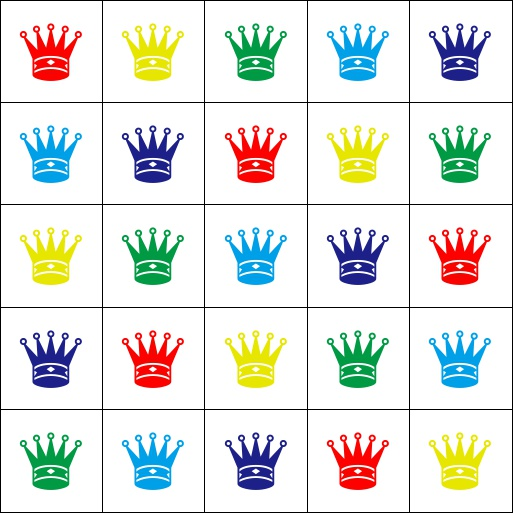
\includegraphics[width=3cm]{images/qgcp_5.jpg}
            \end{column}
            \begin{column}{0.48\textwidth}\centering
                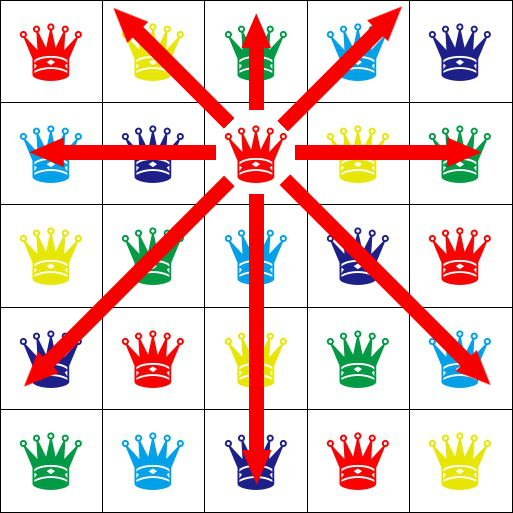
\includegraphics[width=3cm]{images/qgcp_5_c.jpg}
            \end{column}
        \end{columns}
    \end{exampleblock}
    \begin{itemize}
        \item この問題は{\alldifferent}制約のみを用いて記述できる.
        \item Knuthの教科書 The Art of Computer Programming Volume 4 Fascicle 6でも
            取り上げられている~[Knuth '15].
    \end{itemize}
\end{frame}



%%%%%%%%%%%%%%%%%%%%%%%%%%%%%%%%%%%%%%
% alldifferent制約の実装技術
%%%%%%%%%%%%%%%%%%%%%%%%%%%%%%%%%%%%%%
\begin{frame}
    \frametitle{{\alldifferent}制約の実装技術}
    % alldifferent制約はおそらく制約プログラミングにおいて最もよく知られ,最も影響力があり,最も研究されているグローバル制約である.\\
    % これはおそらくマッチング理論との関係によるもので,
    % この理論計算機科学の重要な分野はalldifferent制約に対する効率的なフィルタリングアルゴリズムの基礎を提供した.\\
    マッチング理論はalldifferent制約に対する効率的なフィルタリングアルゴリズムの基礎を提供した.\\

    \begin{block}{マッチング理論に基づく{\alldiff}制約に対するアーク整合性アルゴリズム[Régin]}
        変数の集合$X$,それらのドメインの和を$D(X)$とし,\\
        二部グラフ$G = (X, D(X), E), E = \{\{x, d\} | x \in X, d \in D(x)\}$を表す.
        \[
            x_1 \in \{b, c, d, e\}, x_2 \in \{b, c\}, x_3 \in \{a, b, c, d\}, x_4 \in \{b, c\},
        \]
        \[
            alldifferent(x_1, x_2, x_3, x_4)
        \]
        を考える.
    \end{block}
\end{frame}

% %%%%%%%%%%%%%%%%%%%%%%%%%%%%%%%%%%%%%%
% % alldifferent制約の擬似ブール符号化
% %%%%%%%%%%%%%%%%%%%%%%%%%%%%%%%%%%%%%%
% \begin{frame}
%     \frametitle{{\alldiff}制約の擬似ブール符号化}
%     {\alldiff}制約を$\neq$で表現する他にブール基数制約で表現することができる.
%     \begin{exampleblock}{}
%         $x_i \in \{ 1 \dots d \}, n \geq d$ である $\Alldiff$に対して,$p_{ij}=1 \Llra x_i=j$である$n$行$d$列の0-1行列($p_{ij}$)を導入する.
%         \begin{displaymath}
%             \begin{array}{cccc}
%              & & &
%              \begin{array}{cccc}
%                  1&2&\dots&d
%              \end{array}\\
%                 (p_{ij})&=&
%                 \begin{array}{c}x_1\\ x_2\\ \vdots\\ x_n \end{array}&
%                 \left(
%                     \begin{array}{cccc}
%                         p_{11}&p_{12}&\dots&p_{1d}\\
%                         p_{21}&p_{22}&\dots&p_{2d}\\
%                         \vdots&\vdots&\ddots&\vdots\\
%                         p_{n1}&p_{n2}&\dots&p_{nd}
%                 \end{array}\right)
%             \end{array}
%         \end{displaymath}
%         \begin{itemize}
%             \item 各$x_i$はちょうど一つの値をとる.
%                 % $$ \sum_{j=l}^{u} p_{ij}=1 \; (i \in \{1,2,\ldots,n\}) $$
%             \item 各列について1となるのは高々1つである.
%                 % $$ \sum_{i=1}^{n} p_{ij} \leq 1 \; (j \in \{l,l+1,\ldots,u\})$$
%                 % これは$n=d$の時には等号にできる
%                 % $$\sum_{i=1}^{n} p_{ij} = 1 \; (j \in \{l,l+1,\ldots,u\})$$
%         \end{itemize}
%     \end{exampleblock}
% \end{frame}


%%%%%%%%%%%%%%%%%%%%%%%%%%%%%%%%%%%%%%
% alldifferent制約の直接符号化
%%%%%%%%%%%%%%%%%%%%%%%%%%%%%%%%%%%%%%
\begin{frame}
    \frametitle{{\alldifferent}制約の直接符号化}
    直接符号化法はSAT符号化法の中で最も広く用いられている手法である.
    \begin{alertblock}{直接符号化法(Direct Encoding: DE)}
        各整数変数$x$と各整数定数$a \in \Dom(x)$に対して,$x = a$を意味する命題変数\alert{\bf $\dE{x}{a}$}を用いる.
    \end{alertblock}
    \begin{block}{{\alldifferent}制約を直接符号化法で表す利点}
        \begin{itemize}
            \item {\alldifferent}制約を$\neq$に分解してSAT符号化し,DEと相性の良いat-least-one制約をヒント制約として追加することができる.
            \item {\alldifferent}制約を擬似ブール符号化してからSATに符号化することができる.
        \end{itemize}
    \end{block}
\end{frame}



%%%%%%%%%%%%%%%%%%%%%%%%%%%%%%%%%%%%%%
% 順序符号化
%%%%%%%%%%%%%%%%%%%%%%%%%%%%%%%%%%%%%%
\begin{frame}
    \frametitle{{\alldifferent}制約の順序符号化}
    % \begin{itemize}
    %     \item 2000年以降,命題論理の充足可能性判定問題を解くSAT ソルバーの性能が飛躍的に向上し,{\alldifferent}制約を含む制約充足問題をSAT に符号化して解く手法の研究が進められた.
    % \end{itemize}
    \begin{alertblock}{順序符号化法(Order Encoding: OE)}
        各整数変数$x$と各整数定数$a \in \Dom(x)$に対して,$x \le a$を意味する命題変数\alert{\bf $\oE{x}{a}$}を用いる.
    \end{alertblock}
    \begin{block}{{\alldifferent}制約を順序符号化法で表す利点}
        \begin{itemize}
            \item {\alldifferent}制約を$\neq$に分解してSAT符号化し,OEと相性の良い鳩の巣原理をヒント制約として追加することができる.
        \end{itemize}
    \end{block}
    \begin{itemize}
        \item 順序符号化法に基づいたSAT型制約ソルバーSugarが,2008年国際制約ソルバー競技会のグローバル制約部門で第1位になるなど,{\alldifferent}制約に対して優れた性能を示している.
    \end{itemize}
\end{frame}



%%%%%%%%%%%%%%%%%%%%%%%%%%%%%%%%%%%%%%
% 研究概要
%%%%%%%%%%%%%%%%%%%%%%%%%%%%%%%%%%%%%%
\begin{frame}
    \frametitle{研究概要}
    \begin{alertblock}{研究目的}
        % チャネリング制約を用いて{\alldifferent}制約をSAT符号化し,
        % クイーングラフ彩色問題を題材として比較評価する.
        {\alldifferent}制約を高速化するために新たなSAT符号化を実装し,比較評価する
    \end{alertblock}
    \begin{block}{研究内容}
        \begin{enumerate}
            % \item {\alldifferent}制約の整数変数を直接符号化法(DE)と順序符号化法(OE)のいずれかでSAT符号化
            % \item {\alldifferent}制約の表現方法を4種類実装
            %     \begin{itemize}
            %         \item $\neq$の形に分解
            %         \item {\alldifferent}制約の擬似ブール符号化(基本PB,PB3,PB4)
            %     \end{itemize}
            % \item {\alldifferent}制約の高速化手法を2種類実装
            %     \begin{itemize}
            %         \item 鳩の巣原理を用いたヒント制約(PHP)
            %         \item at-least-one制約を用いたヒント制約(ALT1)
            %     \end{itemize}
            % \item クイーングラフ彩色問題($5\leq N \leq 12$)を用いた評価実験
            % \item OEとDEを融合させるチャネリング制約の実装
            \item 順序符号化法と直接符号化法をチャネリング制約を用いて融合させる手法を実装
            \item クイーングラフ彩色問題($5\leq N \leq 12$)を用いた評価実験
                \begin{itemize}
                    \item チャネリング制約の有無・{\alldifferent}制約の表現方法・{\alldifferent}制約の高速化手法の有無を切り替え,計12符号化を比較した.
                \end{itemize}
        \end{enumerate}
    \end{block}
\end{frame}



%%%%%%%%%%%%%%%%%%%%%%%%%%%%%%%%%%%%%%
% チャネリング制約を用いたalldifferent制約のSAT符号化
%%%%%%%%%%%%%%%%%%%%%%%%%%%%%%%%%%%%%%
\begin{frame}
    \frametitle{チャネリング制約を用いた{\alldifferent}制約のSAT符号化}
    \begin{block}{基本的アイデア}
        各整数変数$x$と各整数定数$a \in \Dom(x)$に対して,順序符号化法(OE)と直接符号化法(DE)の両方の命題変数を導入し,以下のような制約を追加する.
        \footnote{$a-1 \in \Dom(x)$の場合は,$\lnot\oE{x}{a-1}$は省略}
        \[
            \dE{x}{a} \Llra \lnot\oE{x}{a-1} \land \oE{x}{a}
        \]
    \end{block}
    \begin{alertblock}{チャネリング制約を用いる利点}
        \begin{itemize}
            % \item $\Alldiff$を$\land x_i \neq x_j$の形に分解し,各々の$x_i \neq x_j$をOEとDEのいずれかを用いてSAT符号化することができる.
            \item OEで有効性が確認されている鳩の巣原理(PHP)に基づくヒント制約と$n=d$の場合にDEで有効性が確認されているat-least-one制約(ALT1)を組み合わせて利用することができる.
                % \item {\alldifferent}制約を$\land x_i \neq x_j$の形に分解する代わりに,擬似ブール(PB)制約に符号化し,その後,SAT符号化することができる.
        \end{itemize}
    \end{alertblock}
\end{frame}



%%%%%%%%%%%%%%%%%%%%%%%%%%%%%%%%%%%%%%
% 比較に用いたalldifferent制約の符号化一覧
%%%%%%%%%%%%%%%%%%%%%%%%%%%%%%%%%%%%%%
\begin{frame}
    \frametitle{比較に用いた{\alldifferent}制約の符号化一覧}
    \begin{block}{}\centering
        {\tiny  \begin{tabular}[c] {|c|c|c|c|c|}\hline
  model & 符号    & alldiff & PHP & ALT1 \\\hline
  0     & OE      & neq     &    &      \\
  1     & OE      & neq     & \checkmark   &      \\
  2     & OE      & neq     &    & \checkmark    \\
  3     & OE      & neq     & \checkmark   & \checkmark    \\
  4     & OE{\textless=\textgreater}DE & neq     &    &  \\
  5     & OE{\textless=\textgreater}DE & neq     & \checkmark   &  \\
  6     & OE{\textless=\textgreater}DE & neq     &    & \checkmark \\
  7     & OE{\textless=\textgreater}DE & neq     & \checkmark   & \checkmark \\
  8     & OE{\textless=\textgreater}DE & PB      &    &   \\
  9     & OE{\textless=\textgreater}DE & PB      & \checkmark   &   \\
  10    & OE{\textless=\textgreater}DE & 大野3   &    &   \\
  11    & OE{\textless=\textgreater}DE & 大野3   & \checkmark   &   \\
  12    & OE{\textless=\textgreater}DE & 大野4   &    &   \\
  13    & OE{\textless=\textgreater}DE & 大野4   & \checkmark   &   \\\hline
 \end{tabular}
}
    \end{block}
    \begin{itemize}
        \item 3列目以降のDE・ODは直接符号化法と順序符号化法のどちらを用いてSAT符号化するのかを表している.
        \item 符号化1は高速制約ソルバーSugarのデフォルト設定と同じである.
        \item 符号化2-11はチャネリング制約を用いた提案手法である.
        \item 符号化3は先行研究であるI.Gentのものと同じ設定である.
    \end{itemize}
\end{frame}



%%%%%%%%%%%%%%%%%%%%%%%%%%%%%%%%%%%%%%
% 実験概要
%%%%%%%%%%%%%%%%%%%%%%%%%%%%%%%%%%%%%%
\begin{frame}
    \frametitle{実験概要}
    実装したSAT符号化及び{\alldifferent}制約の高速化手法を評価するために,以下の実験を行なった.
    \begin{itemize}
        \item \structure{比較に用いた実装(12個)}
            % \vspace{-3mm}
            % \begin{block}{}\centering
            %     {\fontsize{4pt}{5pt}\selectfont  \begin{tabular}[c] {|c|c|c|c|c|}\hline
  model & 符号    & alldiff & PHP & ALT1 \\\hline
  0     & OE      & neq     &    &      \\
  1     & OE      & neq     & \checkmark   &      \\
  2     & OE      & neq     &    & \checkmark    \\
  3     & OE      & neq     & \checkmark   & \checkmark    \\
  4     & OE{\textless=\textgreater}DE & neq     &    &  \\
  5     & OE{\textless=\textgreater}DE & neq     & \checkmark   &  \\
  6     & OE{\textless=\textgreater}DE & neq     &    & \checkmark \\
  7     & OE{\textless=\textgreater}DE & neq     & \checkmark   & \checkmark \\
  8     & OE{\textless=\textgreater}DE & PB      &    &   \\
  9     & OE{\textless=\textgreater}DE & PB      & \checkmark   &   \\
  10    & OE{\textless=\textgreater}DE & 大野3   &    &   \\
  11    & OE{\textless=\textgreater}DE & 大野3   & \checkmark   &   \\
  12    & OE{\textless=\textgreater}DE & 大野4   &    &   \\
  13    & OE{\textless=\textgreater}DE & 大野4   & \checkmark   &   \\\hline
 \end{tabular}
}
            % \end{block}
        \item \structure{ベンチマーク問題}
            \begin{itemize}
                \item $N$次クイーングラフ彩色問題 ($8\leq N\leq 12$)
            \end{itemize}
        \item \structure{SATソルバー}: Sugar ver.2.3.3 ,GlueMiniSat 2.2.10-193
        \item \structure{制限時間}: 1問あたり2時間\\
            \begin{itemize}
                \item N=12についてはN=11で性能のよかった上位3符号化を制限時間を72時間に伸ばして実験を行った
            \end{itemize}
        \item \structure{実験環境}: Mac mini, 3.2GHz, 64GB メモリ
    \end{itemize}
\end{frame}



%%%%%%%%%%%%%%%%%%%%%%%%%%%%%%%%%%%%%%
% 実験結果
%%%%%%%%%%%%%%%%%%%%%%%%%%%%%%%%%%%%%%
\begin{frame}
    \frametitle{実験結果: 求解に要したCPU時間(秒)}
    \begin{block}{}\centering
        {\tiny \begin{tabular}{l|rr|rr} 
  & \multicolumn{2}{c|}{基本ソルバー} & \multicolumn{2}{c}{改良ソルバー} \\
  & \code{changed} & \code{unchanged} & \code{changed} & \code{unchanged} \\ \hline
  解けた問題数(到達可能) & 11 & 11 & 11 & 11 \\
  解けた問題数(到達不能) & 10 & 10 & 56 & \alert{60} \\\hline
  平均 CPU 時間(秒) & 223.796 & 151.341 & 101.758 & \alert{59.095} \\
\end{tabular}}
    \end{block}
    \begin{itemize}
        \item 既存の順序符号化法のみを用いた手法(符号化 1)よりもチャネリング制約を用いた手法(符号化 2-11)の方が優れている
        \item 解を求めることが困難な$N=12$について符号化 9で求めることができた.
    \end{itemize}
\end{frame}





%%%%%%%%%%%%%%%%%%%%%%%%%%%%%%%%%%%%%%
% まとめ
%%%%%%%%%%%%%%%%%%%%%%%%%%%%%%%%%%%%%%
\begin{frame}
    \frametitle{まとめ}
    \begin{enumerate}
        \item \structure{{\alldifferent}制約に対して,12個の実装方法を提案}
            \begin{itemize}
                % \item 比較のため高速制約ソルバー Sugarのデフォルト設定の手法とチャネリング制約を用いた提案手法に{\alldifferent}制約の高速化手法を合わせて実装した.
                \item 整数変数の符号化方法(OE,OE $\equ$ DE),\\
                    {\alldifferent}制約の表現手法($\neq$分解,基本PB,PB3,PB4)と\\
                    ヒント制約(PHP,ALT1)を組み合わせて実装した.
            \end{itemize}
        \item \structure{クイーングラフ彩色問題($8 \leq N \leq 12$)を用いた評価実験}
            \begin{itemize}
                \item 既存の手法に比べてチャネリング制約の優位性が確認できた.
                \item N=12のクイーングラフ彩色問題において解を求めることができた.
            \end{itemize}
    \end{enumerate}
    \begin{exampleblock}{今後の課題}
        \begin{itemize}
            \item 今回性能の良かった符号化をSugarに組み込む
            \item クイーングラフ彩色問題以外で実験を回す
        \end{itemize}
    \end{exampleblock}
\end{frame}


%%%%%%%%%%%%%%%%%%%%%%%%%%%%%%%%%%%%%%
% 12次クイーングラフ彩色問題の解
%%%%%%%%%%%%%%%%%%%%%%%%%%%%%%%%%%%%%%
\begin{frame}
    \frametitle{12次クイーングラフ彩色問題の解}
    \begin{exampleblock}{}\centering
        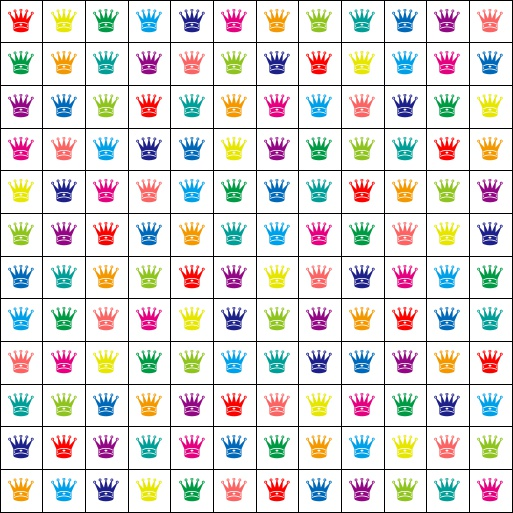
\includegraphics[width=5cm]{images/qgcp_12.jpg}
    \end{exampleblock}
\end{frame}
% %%%% 補助スライド


%%%%%%%%%%%%%%%%%%%%%%%%%%%%%%%%%%%%%%%%%%%%%%%%%%%%%%%%%%%%%
% %%%% 補助スライド
%%%%%%%%%%%%%%%%%%%%%%%%%%%%%%%%%%%%%%%%%%%%%%%%%%%%%%%%%%%%%

\appendix

\backupbegin

%%%%%%%%%%%%%%%%%%%%%%%%%%%%%%%%%%%%%%
% ~
%%%%%%%%%%%%%%%%%%%%%%%%%%%%%%%%%%%%%%
\begin{frame}
    \frametitle{~}
    \centering
    - 補足用 -
\end{frame}



%%%%%%%%%%%%%%%%%%%%%%%%%%%%%%%%%%%%%%
% 鳩の巣原理を用いたヒント制約(PHP)~[田島・田村,2008]
%%%%%%%%%%%%%%%%%%%%%%%%%%%%%%%%%%%%%%
\begin{frame}
    \frametitle{鳩の巣原理を用いたヒント制約(PHP)~[田島・田村,2008]}
    SAT符号化された{\alldifferent}制約に,鳩の巣原理を用いたヒントを加える
    と求解速度が向上することが知られている.
    \begin{block}{}
        $alldifferent(x_{1},\ldots,x_{n})$について,$x_i \in
        \{\ell,\ell+1,\ldots,u\}$であるとき,以下の2つの制約を追加する.
        \[
            \bigvee_{i=1}^{n}x_{i}\geq \ell+n-1 \qquad
            \bigvee_{i=1}^{n}x_{i}\leq u-n+1
        \]
    \end{block}
    \begin{exampleblock}{例}
        $alldifferent(x_1, x_2, x_3)$について, $x_i \in \{1,2,3\}$であるとき,以下の制約が追加される.
        \vspace{-3mm}
        \begin{eqnarray*}
            (x_1\geq 3) \lor (x_2 \geq 3) \lor (x_3 \geq 3)\\
            (x_1\leq 1) \lor (x_2 \leq 1) \lor (x_3 \leq 1)
        \end{eqnarray*}
    \end{exampleblock}
\end{frame}


%%%%%%%%%%%%%%%%%%%%%%%%%%%%%%%%%%%%%%
% at-least-one制約
%%%%%%%%%%%%%%%%%%%%%%%%%%%%%%%%%%%%%%
\begin{frame}
    \frametitle{at-least-one制約を用いたヒント制約(ALT1)}
    \vspace{-3mm}
    \begin{block}{}
        $alldfifferent(x_1,x_2,\ldots,x_n)$について, $x_i \in \{\ell, \ell+1,\ldots, u\}$かつ$u-\ell=n-1$であるときに以下の制約を追加する.\\
        \vspace{-3mm}
        $$\bigvee_{i=1}^n x_i=a \qquad (a \in \{\ell,\ldots, u\})$$
    \end{block}
    \begin{exampleblock}{at-least-one制約を用いたヒント制約の例}
        $alldifferent(x_1, x_2, x_3, x_4)$について, $x_i \in \{1, 2, 3, 4\}$であるときには以下の制約が追加される.
        \vspace{-3mm}
        \begin{eqnarray*}
            (x_1=1) \lor (x_2=1) \lor (x_3=1) \lor (x_4=1)\\
            (x_1=2) \lor (x_2=2) \lor (x_3=2) \lor (x_4=2)\\
            (x_1=3) \lor (x_2=3) \lor (x_3=3) \lor (x_4=3)\\
            (x_1=4) \lor (x_2=4) \lor (x_3=4) \lor (x_4=4)
        \end{eqnarray*}
    \end{exampleblock}
\end{frame}


%%%%%%%%%%%%%%%%%%%%%%%%%%%%%%%%%%%%%%
% alldifferent制約の擬似ブール符号化
%%%%%%%%%%%%%%%%%%%%%%%%%%%%%%%%%%%%%%
\begin{frame}
    \frametitle{{\alldiff}制約の擬似ブール符号化(PB)}
    {\alldiff}制約をブール基数制約で表現することができる.
    \begin{exampleblock}{}
        $x_i \in \{ 1 \dots d \}, n \geq d$ である $\Alldiff$に対して,$p_{ij}=1 \Llra x_i=j$である$n$行$d$列の0-1行列($p_{ij}$)を導入する.
        \vspace{-3mm}
        \begin{displaymath}
            \begin{array}{cccc}
             & & &
             \begin{array}{cccc}
                 1&2&\dots&d
             \end{array}\\
                (p_{ij})&=&
                \begin{array}{c}x_1\\ x_2\\ \vdots\\ x_n \end{array}&
                \left(
                    \begin{array}{cccc}
                        p_{11}&p_{12}&\dots&p_{1d}\\
                        p_{21}&p_{22}&\dots&p_{2d}\\
                        \vdots&\vdots&\ddots&\vdots\\
                        p_{n1}&p_{n2}&\dots&p_{nd}
                \end{array}\right)
            \end{array}
        \end{displaymath}
        \begin{itemize}
            \item 各$x_i$はちょうど一つの値をとる.
            \vspace{-3mm}
                % $$ \sum_{j=1}^{d} p_{ij}=1 \; (i \in \{1,2,\ldots,n\}) $$
            $$ p_{i1} + \ldots + p_{id} = 1 \; (i \in \{1,2,\ldots,n\})$$
            \item 各列について1となるのは高々1つである.
            \vspace{-3mm}
            $$ p_{1j} + \ldots + p_{nj} \leq 1 \; (j \in \{1,2,\ldots,d\})$$
                % $$ \sum_{i=1}^{n} p_{ij} \leq 1 \; (j \in \{l,l+1,\ldots,u\})$$
                % これは$n=d$の時には等号にできる
                % $$\sum_{i=1}^{n} p_{ij} = 1 \; (j \in \{l,l+1,\ldots,u\})$$
        \end{itemize}
    \end{exampleblock}
\end{frame}

%%%%%%%%%%%%%%%%%%%%%%%%%%%%%%%%%%%%%%
% PB3
%%%%%%%%%%%%%%%%%%%%%%%%%%%%%%%%%%%%%%
\begin{frame}
    \frametitle{PB3}
    {\alldiff}制約をブール基数制約
    \begin{exampleblock}{}
        $x_i \in \{ 1 \dots d \}, n \geq d$ である $\Alldiff$に対して,$p_{ij}=1 \Llra x_i=j$である$n$行$d$列の0-1行列($p_{ij}$)を導入する.
        \vspace{-3mm}
        \begin{displaymath}
            \begin{array}{cccc}
             & & &
             \begin{array}{cccc}
                 1&2&\dots&d
             \end{array}\\
                (p_{ij})&=&
                \begin{array}{c}x_1\\ x_2\\ \vdots\\ x_n \end{array}&
                \left(
                    \begin{array}{cccc}
                        p_{11}&p_{12}&\dots&p_{1d}\\
                        p_{21}&p_{22}&\dots&p_{2d}\\
                        \vdots&\vdots&\ddots&\vdots\\
                        p_{n1}&p_{n2}&\dots&p_{nd}
                \end{array}\right)
            \end{array}
        \end{displaymath}
        \begin{itemize}
            \item 各$x_i$はちょうど一つの値をとる.
            \vspace{-3mm}
                % $$ \sum_{j=1}^{d} p_{ij}=1 \; (i \in \{1,2,\ldots,n\}) $$
            $$ p_{i1} + \ldots + p_{id} = 1 \; (i \in \{1,2,\ldots,n\})$$
            \item 各列について1となるのは高々1つである.
            \vspace{-3mm}
            $$ p_{1j} + \ldots + p_{nj} \leq 1 \; (j \in \{1,2,\ldots,d\})$$
                % $$ \sum_{i=1}^{n} p_{ij} \leq 1 \; (j \in \{l,l+1,\ldots,u\})$$
                % これは$n=d$の時には等号にできる
                % $$\sum_{i=1}^{n} p_{ij} = 1 \; (j \in \{l,l+1,\ldots,u\})$$
        \end{itemize}
    \end{exampleblock}
\end{frame}

\backupend

%%% Local Variables:
%%% mode: japanese-latex
%%% TeX-master: "slide"
%%% End:

\end{document}
